\section{Planar Graphs}
\begin{definition}\label{3.1}
    A \textbf{planar drawing} of a graph $G$ consists of injective continuous functions 
    \begin{align*}
        &\phi_v:V(G)\to\mathbb{R}^2 &\phi_e:[0,1]\to\mathbb{R}^2
    \end{align*} s.t.:
    \begin{itemize}
        \item $\{\phi_{\{u,v\}}(0),\phi_{\{u,v\}}(1)\}=\{\phi_u(u),\phi_v(v)\} $ for all $\{u,v\}\in E(G)$
        \item The sets $\phi_e((0,1))$ for each $e\in E(G)$ are pairwise disjoint and disjoint from $\operatorname{Im}(\phi_v)$ (i.e. no crossings)
    \end{itemize} 
    A graph $G$ is called \textbf{planar} if it has a planar drawing.\\
    A \textbf{plane graph} is a planar graph, together with a fixed planar drawing.
\end{definition}
\vspace{0.5cm}
\begin{example}\label{3.2}
\hfill
    \begin{itemize}
        \item Trees
        \item $K_4$
        \item $K_{2,3}$
    \end{itemize}
    \begin{center}
        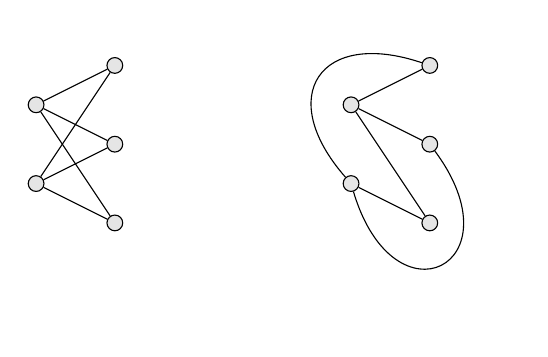
\begin{tikzpicture}[
            vertex/.style={circle, draw, fill=gray!20, minimum size=2mm, inner sep=0pt}
        ]
            \node[vertex] (a1) at (-2, 0.5) {};
            \node[vertex] (a2) at (-2, 1.5) {};
            \node[vertex] (b1) at (-1,   0) {};
            \node[vertex] (b2) at (-1,   1) {};
            \node[vertex] (b3) at (-1,   2) {};
            \draw (a1)--(b1) (a1)--(b2) (a1)--(b3);
            \draw (a2)--(b1) (a2)--(b2) (a2)--(b3);

             \node[vertex] (a1) at (2, 0.5) {};
            \node[vertex] (a2) at (2, 1.5) {};
            \node[vertex] (b1) at (3,   0) {};
            \node[vertex] (b2) at (3,   1) {};
            \node[vertex] (b3) at (3,   2) {};
            \draw (a1)--(b1); 
            \draw (a1) to [bend right=100, looseness=4](b2); 
            \draw (a1) to [bend left=75, looseness=2](b3);
            \draw (a2)--(b1) (a2)--(b2) (a2)--(b3);
        \end{tikzpicture}
        \end{center}
\end{example}
\vspace{0.5cm}
\begin{definition}\label{3.3}
    A \textbf{face} of a plane graph $G$ is a maximal connected part of $\mathbb{R}^2\backslash(\operatorname{Im}(\phi_v(u))\cup \operatorname{Im}(\phi_e))$. Every plane graph has exactly one unbounded face called the \textbf{outer face}. All other faces are called \textbf{inner faces}. The \textbf{boundary} of a face are the vertices and edges of $G$ incident with it. A plane graph is called \textbf{planar triangulation} if every face is bounded by a cycle of length precisely 3 (this includes the outer face).
\end{definition}
\vspace{0.5cm}
\begin{theorem}[Euler's formula]\label{3.4}
    Let $G=(V,E)$ be a connected planar graph. Then the number of faces $|F|$ of $G$ is $|F|=|E|-|V|+2$.
\end{theorem}
\begin{proof}
    Induction on $|E|$. \\
    Since $G$ is connected, we have $|E|\geq|V|-1$ so we start the induction at $|E|=|V|-1\implies G$ is a tree. Since a tree does not contain a cycle, we have $|F|=|E|-|V|+2$. \\
    Now let $|E|>|V|-1$. Then $G$ is not a tree, so $G$ contains a cycle $C$. Choose an edge $e$ on $C$ and remove it to obtain a plane graph $G'$. $e$ separates two faces in $G$, which fuse to a single face in $G'$. By induction, the number of faces $|F'|$ in $G'$ is $|F|-1=|F'|=|E|-1-|V|+2\implies|F|=|E|-|V|+2$.
\end{proof}
\vspace{2cm}
\begin{lemma}\label{3.5}
    For every plane graph $G=(V,E)$ with $|V|\geq3$, we have $|E|\leq3|V|-6$.
\end{lemma}
\begin{proof}
    Wlog $G$ is connected. Consider a planar drawing of $G$ and let $F$ be the set of faces. Every face is bounded by at least $3$ edges and each edge bounds at most $2$ faces. By Euler's formula \ref{3.4}, we obtain $\frac{2}{3}|E|\geq|F|=|E|-|V|+2\implies|E|\leq3|V|-6$. 
\end{proof}
\begin{remark}\label{3.6}
    This means that the number of edges in a planar graph grows only linear proportional to the number of vertices. 
\end{remark}
\vspace{0.5cm}
\begin{example}\label{3.7}
    \hfill\begin{itemize}
        \item $K_5$ is not planar ($10$ edges) due to Theorem \ref{3.4}
        \item $K_{3,3}$ is not planar (without proof)
    \end{itemize}
\end{example}
\vspace{0.5cm}
\begin{definition}\label{3.8}
    A \textbf{subdivision} of a graph $G$ is a graph obtained from $G$ by repeatedly subdividing some of its edges.
\end{definition}
\vspace{0.5cm}
\begin{theorem}[Kuratowski's theorem]\label{3.9}
    A graph $G$ is planar iff $G$ contains no subgraph that is a subdivision of $K_5$ or $K_{3,3}$.
\end{theorem}
\begin{remark}\label{3.10}
    A subdivision of a graph is planar iff the graph is planar
\end{remark}
\vspace{0.5cm}
\begin{definition}\label{3.11}
    Let $G$ be a graph. The graph obtained from $G$ by contracting $e=\{u,v\}\in E(G)$ denoted $G/e$, is the graph obtained from $G$ by deleting $u,v$, inserting a new vertex $w$ and making $w$ adjacent to all vertices in $N_G(u)\cup N_G(v)$.\\
    A graph $G'$ is a \textbf{minor} of $G$ if $G'$ can be obtained from $G$ by a sequence of vertex deletions, edge deletions and edge contractions.
\end{definition}
\begin{remark}\label{3.12}
    If $G'$ is a minor of $G$ then $G'$ planar $\impliedby G$ is planar.
\end{remark}
\vspace{0.5cm}
\begin{theorem}[Wagner's theorem]\label{3.13}
    A graph $G$ is planar iff $K_{3,3}$ and $K_5$ are not a minor of $G$.
\end{theorem}